\documentclass[runningheads]{llncs}
\usepackage[T1]{fontenc}
\usepackage{graphicx}
\usepackage{amsmath,amssymb}
\usepackage{booktabs}
\usepackage{xcolor}
\usepackage{hyperref}
\renewcommand{\UrlFont}{\rmfamily}

\emergencystretch=1em
\begin{document}

\title{Trustworthy MRI Reconstruction via Conformal Prediction\\and K-Space Data Consistency}
\titlerunning{Trustworthy MRI via CP and K-Space Consistency}

\author{Baljinnyam Dayan}
\authorrunning{Dayan}
\institute{Imperial College London, London, UK\\\email{bd1125@ic.ac.uk}\\CID: 06059151}

\maketitle

\begin{abstract}
    Deep learning MRI reconstruction provides no reliability guarantees, a critical limitation for clinical deployment. We address this through \emph{split conformal prediction} for pixel-wise intervals with distribution-free marginal coverage guarantees, extended with \emph{adaptive} intervals using gradient magnitude as a spatial difficulty modulator, and \emph{k-space data consistency residuals} as a physics-informed check on range-space consistency with acquired measurements. On fastMRI proton-density knees, conformal prediction achieves near-exact $90\%$ coverage at $4{\times}$ and $8{\times}$ acceleration (where MC Dropout, at the dropout rate used for reconstruction, achieves ${\sim}55\%$), and adaptive intervals reduce median width by ${\sim}15\%$ compared to uniform intervals. K-space residuals correlate with reconstruction errors ($r{=}0.39$ at $4{\times}$), providing a complementary trustworthiness signal.

    \keywords{MRI reconstruction \and Conformal prediction \and Uncertainty quantification \and Data consistency \and Trustworthy AI}
\end{abstract}

%----------------------------------------------------------------------
\section{Introduction}
%----------------------------------------------------------------------

Accelerated MRI reduces scan time by acquiring fewer k-space measurements, relying on reconstruction algorithms to recover diagnostic-quality images. Deep learning approaches~\cite{ronneberger2015unet,hammernik2018varnet,sriram2020e2evarnet,schlemper2018cascade} have dramatically improved reconstruction quality, but provide point estimates with no indication of reliability---a fundamental barrier to clinical trust.

At high acceleration (e.g., $8{\times}$), substantial detail must be inferred from limited measurements, risking hallucinated structures~\cite{bhadra2021hallucinations}. Existing uncertainty methods---MC Dropout~\cite{gal2016dropout}, deep ensembles~\cite{lakshminarayanan2017ensembles}---produce useful maps but offer no formal coverage guarantees. Conformal prediction~\cite{shafer2008tutorial,angelopoulos2023gentle} fills this gap with \emph{distribution-free} guarantees, but pixel-level application to MRI reconstruction remains underexplored.

We make the following contributions:\footnote{Code and reproducibility assets: \href{https://github.com/baljinnyamday/trustworthy-MRI-reconstruction}{github.com/baljinnyamday/trustworthy-MRI-reconstruction}}
\begin{enumerate}
    \item Split conformal prediction for pixel-wise MRI reconstruction intervals with marginal coverage guarantees at $4{\times}$ and $8{\times}$, extended with \emph{adaptive} intervals using gradient magnitude as a spatial difficulty modulator.
    \item K-space data consistency residuals as a physics-informed range-space consistency check, complementing CP's statistical guarantees with a spatial error signal.
    \item Empirical comparison showing conformal prediction achieves its marginal coverage target where MC Dropout---at the dropout rate ($p{=}0.05$) needed for competitive reconstruction quality---undercovers by ${\sim}35$ percentage points, illustrating the value of distribution-free guarantees.
\end{enumerate}

%----------------------------------------------------------------------
\section{Related Work}
%----------------------------------------------------------------------

\paragraph{MRI reconstruction.} U-Net~\cite{ronneberger2015unet} is the standard baseline; stronger architectures include variational networks~\cite{hammernik2018varnet}, end-to-end VarNet~\cite{sriram2020e2evarnet}, and cascaded CNNs with data consistency~\cite{schlemper2018cascade}. We use U-Net since our focus is trustworthiness, not architecture; moreover, stronger models such as E2E-VarNet require multi-coil complex-valued k-space, whereas our single-coil magnitude setting matches the standard fastMRI benchmark. Our CP and k-space methods are model-agnostic and would transfer to any backbone.

\paragraph{Uncertainty quantification.} MC Dropout~\cite{gal2016dropout} and deep ensembles~\cite{lakshminarayanan2017ensembles} produce useful uncertainty maps but are systematically miscalibrated~\cite{kuleshov2018calibration}. K\"ustner et al.~\cite{kustner2024ensembles} showed on fastMRI that ensemble uncertainty correlates with error but coverage still deviates from nominal levels. None of these methods guarantee that a stated $90\%$ interval actually covers $90\%$ of the time.

\paragraph{Conformal prediction.} Conformal prediction~\cite{shafer2008tutorial,angelopoulos2023gentle} provides distribution-free coverage guarantees requiring only exchangeability. Angelopoulos et al.~\cite{angelopoulos2022image} extended it to image regression with learned nonconformity scores that adapt interval width spatially, but require training an auxiliary model. We propose a training-free alternative using gradient magnitude. In medical imaging, Kutiel et al.~\cite{kutiel2023masks} proposed binary reliable/unreliable region masks, and Fischer et al.~\cite{fischer2025cute} used conformalised intervals \emph{during} acquisition to guide adaptive k-space sampling decisions---the closest work to ours, but fundamentally different in scope: their intervals inform the acquisition process in real time, whereas ours provide post-hoc assessment of a completed reconstruction. No prior work combines pixel-level conformal prediction with physics-informed consistency for post-hoc MRI reconstruction assessment.

\paragraph{Hallucination detection.} Bhadra et al.~\cite{bhadra2021hallucinations} formalised hallucinations through null-space analysis: components invisible to acquired measurements can be fabricated without detectable inconsistency. Our k-space consistency metric (Section~\ref{sec:kspace}) is complementary, detecting \emph{range-space} inconsistency where reconstructions disagree with data that \emph{was} measured. While data consistency layers are standard \emph{inside} reconstruction networks~\cite{hammernik2018varnet,schlemper2018cascade}, their use as a standalone post-hoc trustworthiness metric is underexplored.

%----------------------------------------------------------------------
\section{Methods}
%----------------------------------------------------------------------

\subsection{Problem Formulation and Baseline}

Accelerated MRI acquires undersampled k-space $\mathbf{y} = \mathbf{M}\mathcal{F}\mathbf{x} + \boldsymbol{\epsilon}$, where $\mathbf{M}$ retains $1/R$ of k-space lines ($c{=}0.08$ central lines always acquired). The zero-filled input $\mathbf{x}_\text{zf} = \mathcal{F}^{-1}(\mathbf{M}^\top \mathbf{y})$ is fed to a learned reconstruction $\hat{\mathbf{x}} = f_\theta(\mathbf{x}_\text{zf})$.

We use a standard U-Net~\cite{ronneberger2015unet} (${\sim}7.7$M parameters, dropout $p{=}0.05$) trained with $\mathcal{L} = 0.5\,\|\hat{\mathbf{x}} - \mathbf{x}\|_1 + 0.5\,(1 - \text{SSIM}(\hat{\mathbf{x}}, \mathbf{x}))$ using AdamW ($\text{lr}{=}10^{-3}$).

\subsection{Conformal Prediction for MRI Reconstruction}
\label{sec:conformal}

We apply split conformal prediction~\cite{shafer2008tutorial,angelopoulos2023gentle} at the pixel level. Given a held-out calibration set $\{(\mathbf{x}_\text{zf}^{(i)}, \mathbf{x}^{(i)})\}_{i=1}^{n}$ disjoint from training data, we compute per-pixel nonconformity scores:
\begin{equation}
    s^{(i)}_{j} = |\hat{x}^{(i)}_j - x^{(i)}_j|, \quad j = 1, \ldots, HW.
    \label{eq:scores}
\end{equation}

For target miscoverage rate $\alpha \in (0,1)$, the conformal quantile $\hat{q}$ is the $\lceil (1{-}\alpha)(n'{+}1) \rceil / n'$ empirical quantile of the pooled scores $\{s^{(i)}_j\}$, where $n' = nHW$. At test time, the prediction interval at pixel $j$ is:
\begin{equation}
    C_j(\hat{\mathbf{x}}) = [\hat{x}_j - \hat{q},\; \hat{x}_j + \hat{q}].
    \label{eq:interval}
\end{equation}

\paragraph{Coverage guarantee.} Since we pool all pixels from all calibration images, the exchangeability unit is a \emph{pixel}, and split conformal prediction guarantees marginal coverage over a randomly drawn test pixel~\cite{angelopoulos2023gentle}:
\begin{equation}
    \mathbb{P}\!\bigl(x_j \in C_j(\hat{\mathbf{x}})\bigr) \geq 1 - \alpha,
    \label{eq:guarantee}
\end{equation}
where the probability is over the joint draw of calibration set and test pixel. This does \emph{not} guarantee per-image coverage---individual images may deviate (see Section~\ref{sec:discussion})---but holds on average regardless of model quality or data distribution. The intervals are uniform---every pixel receives the same $\hat{q}$---which is unnecessarily conservative in smooth regions.

\subsection{Adaptive Conformal Prediction}
\label{sec:adaptive}

Following Angelopoulos et al.~\cite{angelopoulos2022image}, we replace the absolute residual with a normalised score:
\begin{equation}
    s^{(i)}_j = \frac{|\hat{x}^{(i)}_j - x^{(i)}_j|}{\max(\sigma^{(i)}_j, \epsilon)},
    \label{eq:adaptive_score}
\end{equation}
where $\sigma^{(i)}_j$ is a per-pixel difficulty estimate and $\epsilon{=}10^{-3}$ prevents division by zero.

\paragraph{Gradient magnitude as difficulty modulator.} We use the reconstruction's gradient magnitude as a spatial difficulty estimate:
\begin{equation}
    \sigma^{(i)}_j = \left(\sqrt{(G_x \hat{x}^{(i)})_j^2 + (G_y \hat{x}^{(i)})_j^2} + \epsilon\right)^{\!\gamma},
    \label{eq:grad_sigma}
\end{equation}
where $G_x, G_y$ are Sobel operators applied after light Gaussian smoothing ($\sigma_\text{smooth}{=}1$), and $\gamma{=}0.3$ compresses the dynamic range to prevent excessively wide intervals at strong edges. This requires no additional inference or training. The adaptive interval at pixel $j$ becomes:
\begin{equation}
    C_j^\text{adapt}(\hat{\mathbf{x}}) = [\hat{x}_j - \hat{q}_\text{adapt}\cdot\sigma_j,\; \hat{x}_j + \hat{q}_\text{adapt}\cdot\sigma_j].
    \label{eq:adaptive_interval}
\end{equation}
The conformal guarantee in Eq.~\eqref{eq:guarantee} is preserved because the normalised scores remain exchangeable.

\subsection{K-Space Data Consistency}
\label{sec:kspace}

Given a reconstruction $\hat{\mathbf{x}}$ and measurements $\mathbf{y}$, the k-space residual is:
\begin{equation}
    \mathbf{r} = \mathbf{M} \odot (\mathcal{F}\hat{\mathbf{x}} - \mathbf{y}).
    \label{eq:residual}
\end{equation}
The image-domain residual $\mathbf{r}_\text{img} = |\mathcal{F}^{-1}(\mathbf{r})|$ provides a spatial consistency map. We define a scalar consistency score $\text{CS}(\hat{\mathbf{x}}, \mathbf{y}, \mathbf{M}) = \|\mathbf{r}\|_2 / \|\mathbf{M} \odot \mathbf{y}\|_2$, where $\text{CS}{=}0$ indicates perfect consistency with measured data.

\subsection{MC Dropout Baseline}
\label{sec:mcdropout}

We compare against MC Dropout~\cite{gal2016dropout} ($T$ stochastic passes, intervals from $\hat{\mu}_j \pm z_{\alpha/2}\hat{\sigma}_j$), which carries no formal coverage guarantee.

%----------------------------------------------------------------------
\section{Experiments}
%----------------------------------------------------------------------

\subsection{Dataset and Setup}

We use the fastMRI PD knee dataset~\cite{zbontar2018fastmri}: single-coil $320{\times}320$ magnitude images, 9{,}680 training and 2{,}000 validation slices. Retrospective Cartesian undersampling at $4{\times}$ and $8{\times}$ retains 8\% central k-space lines. Separate U-Nets are trained per acceleration for 30 epochs (AdamW, $\text{lr}{=}10^{-3}$, batch 16) on NVIDIA T4 GPU. The validation set is split by MRI volume into disjoint calibration (50\%) and test (50\%) partitions, preventing leakage through correlated slices. MC Dropout uses $T{=}20$ passes.

\subsection{Reconstruction Quality}

Table~\ref{tab:results} summarises all results. The U-Net achieves 32.01\,dB PSNR / 0.827 SSIM at $4{\times}$, degrading to 30.08\,dB / 0.773 at $8{\times}$.

\begin{table}[t]
    \centering
    \caption{Evaluation results at $4{\times}$ and $8{\times}$ acceleration over 1{,}000 test images. Coverage at nominal 90\%. Adaptive CP uses gradient magnitude as the difficulty modulator ($\gamma{=}0.3$). Adaptive width shown as mean (median).}
    \label{tab:results}
    \begin{tabular}{lccccccccc}
        \toprule
                  & \multicolumn{2}{c}{Recon.} & \multicolumn{2}{c}{Uniform CP} & \multicolumn{2}{c}{Adaptive CP} & \multicolumn{2}{c}{MC Drop.} & KS                                              \\
        \cmidrule(lr){2-3} \cmidrule(lr){4-5} \cmidrule(lr){6-7} \cmidrule(lr){8-9} \cmidrule(lr){10-10}
        Accel.    & PSNR                       & SSIM                           & Cov.                            & Width                        & Cov.   & Width         & Cov.   & Width & Corr. \\
        \midrule
        $4\times$ & 32.01                      & .827                           & 89.8\%                          & 0.462                        & 89.6\% & 0.424 (0.393) & 57.5\% & 0.188 & 0.389 \\
        $8\times$ & 30.08                      & .773                           & 89.7\%                          & 0.560                        & 89.6\% & 0.501 (0.470) & 52.4\% & 0.189 & 0.280 \\
        \bottomrule
    \end{tabular}
\end{table}

\subsection{Conformal Prediction Results}

At nominal 90\% coverage, conformal prediction achieves 89.8\% and 89.7\% empirical coverage at $4{\times}$ and $8{\times}$ respectively, nearly exact. The conformal quantiles are $\hat{q}{=}0.231$ ($4{\times}$) and $\hat{q}{=}0.280$ ($8{\times}$), with wider intervals at higher acceleration correctly reflecting greater uncertainty.

\paragraph{Calibration and per-image coverage.} Figure~\ref{fig:calibration}(a) compares calibration curves across nominal levels from 50\% to 99\%. Conformal prediction tracks the ideal diagonal, deviating by at most 0.3 percentage points (e.g., 99\% $\to$ 99.0\%, 90\% $\to$ 89.8\%). MC Dropout undercovers at every level, with the gap widening at higher coverage: at 99\% nominal it achieves only 72.3\% empirical. We note that our dropout rate ($p{=}0.05$) was chosen for reconstruction quality; higher rates would increase variance estimates but degrade the reconstruction itself---an inherent trade-off in MC Dropout where a single $p$ must serve both purposes~\cite{gal2016dropout}.

While conformal prediction guarantees \emph{marginal} coverage, individual images may vary. Figures~\ref{fig:calibration}(b,c) show per-image coverage across 1{,}000 test images: mean 89.8\% ($\sigma{=}4.6\%$, 5th percentile 81.1\%) at $4{\times}$ and 89.7\% ($\sigma{=}4.0\%$, 5th percentile 82.1\%) at $8{\times}$, though a minority of anatomically complex slices fall well below nominal (Section~\ref{sec:discussion}).

\begin{figure}[t]
    \centering
    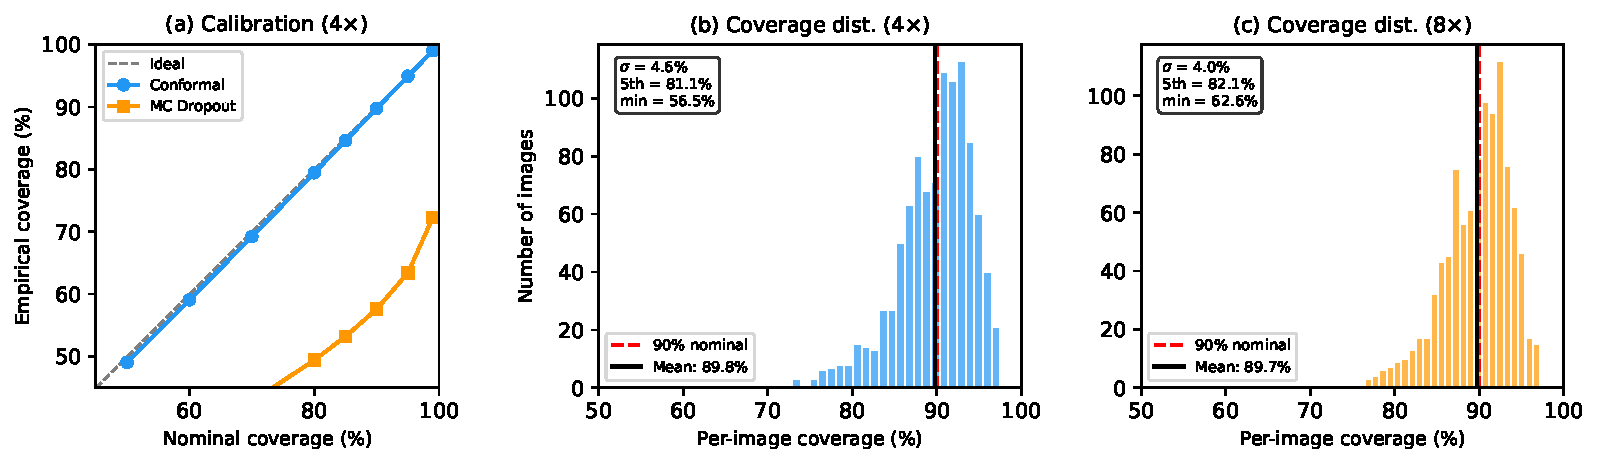
\includegraphics[width=\textwidth]{figures/fig_calibration_and_coverage.pdf}
    \caption{Conformal prediction reliability. (a) Calibration: CP (blue) tracks the ideal diagonal while MC Dropout (orange) severely undercovers. (b,c) Per-image coverage distribution (1{,}000 test images) at $4{\times}$ and $8{\times}$; most images cluster near 90\% nominal, with a tail of undercovered slices.}
    \label{fig:calibration}
\end{figure}

\subsection{Adaptive Conformal Prediction Results}

Adaptive conformal prediction achieves 89.6\% and 89.6\% empirical coverage at $4{\times}$ and $8{\times}$---matching uniform CP's empirical marginal coverage---while substantially reducing interval width in smooth regions. The adaptive quantile is $\hat{q}_\text{adapt}{=}0.305$ ($4{\times}$), applied as a multiplier on the per-pixel gradient magnitude $\sigma_j$ (Eq.~\ref{eq:grad_sigma}).

\paragraph{Interval efficiency.} Figure~\ref{fig:adaptive} compares uniform and adaptive intervals on the same slice. Uniform intervals assign constant width 0.462 across all pixels. Adaptive intervals concentrate width at anatomical boundaries while reducing it in smooth regions, with a median width of 0.393---a 14.9\% reduction from uniform. The mean width is 0.424, reflecting the wider intervals allocated to difficult edge pixels. At $8{\times}$, the reduction is similar: median width drops from 0.560 to 0.470 (16.1\% reduction).

\paragraph{Sensitivity to $\gamma$ and conditional coverage.} Table~\ref{tab:gamma_ablation} shows how $\gamma$ affects both interval efficiency (median width) and fairness (smooth--edge coverage gap, classified by per-image median gradient threshold). Lower $\gamma$ compresses the gradient range more aggressively; higher $\gamma$ approaches raw gradient magnitude and causes extreme widths at edges. Among the values tested, $\gamma{=}0.3$ achieves the lowest median width while nearly eliminating the coverage gap between smooth regions and anatomical boundaries (0.2\,pp at $4{\times}$ vs.\ 13.5\,pp for uniform CP).

\begin{table}[t]
    \centering
    \caption{Adaptive CP ablation over $\gamma$ (90\% nominal). Median width measures interval efficiency; Gap is the smooth--edge coverage difference in percentage points (positive = edges undercovered).}
    \label{tab:gamma_ablation}
    \label{tab:region_coverage}
    \begin{tabular}{@{}l@{\;\;}c@{\;\;}c@{\;\;}r@{\qquad}c@{\;\;}c@{\;\;}r@{}}
        \toprule
                       & \multicolumn{3}{c}{$4\times$} & \multicolumn{3}{c}{$8\times$}                                         \\
        \cmidrule(lr){2-4} \cmidrule(l){5-7}
                       & Cov.                          & Med.\ W.                      & Gap     & Cov.   & Med.\ W. & Gap     \\
        \midrule
        Uniform        & 89.8\%                        & 0.462                         & 13.5    & 89.7\% & 0.560    & 14.6    \\
        \addlinespace
        $\gamma{=}0.1$ & 89.7\%                        & 0.426                         & 10.1    & 89.7\% & 0.514    & 11.8    \\
        $\gamma{=}0.2$ & 89.6\%                        & 0.403                         & 5.6     & 89.6\% & 0.483    & 7.9     \\
        $\gamma{=}0.3$ & 89.6\%                        & 0.393                         & 0.2     & 89.6\% & 0.470    & 2.7     \\
        $\gamma{=}0.5$ & 89.6\%                        & 0.422                         & $-$10.7 & 89.6\% & 0.504    & $-$9.3  \\
        $\gamma{=}1.0$ & 89.9\%                        & 0.801                         & $-$19.8 & 89.9\% & 0.965    & $-$19.8 \\
        \bottomrule
    \end{tabular}
\end{table}

\begin{figure}[t]
    \centering
    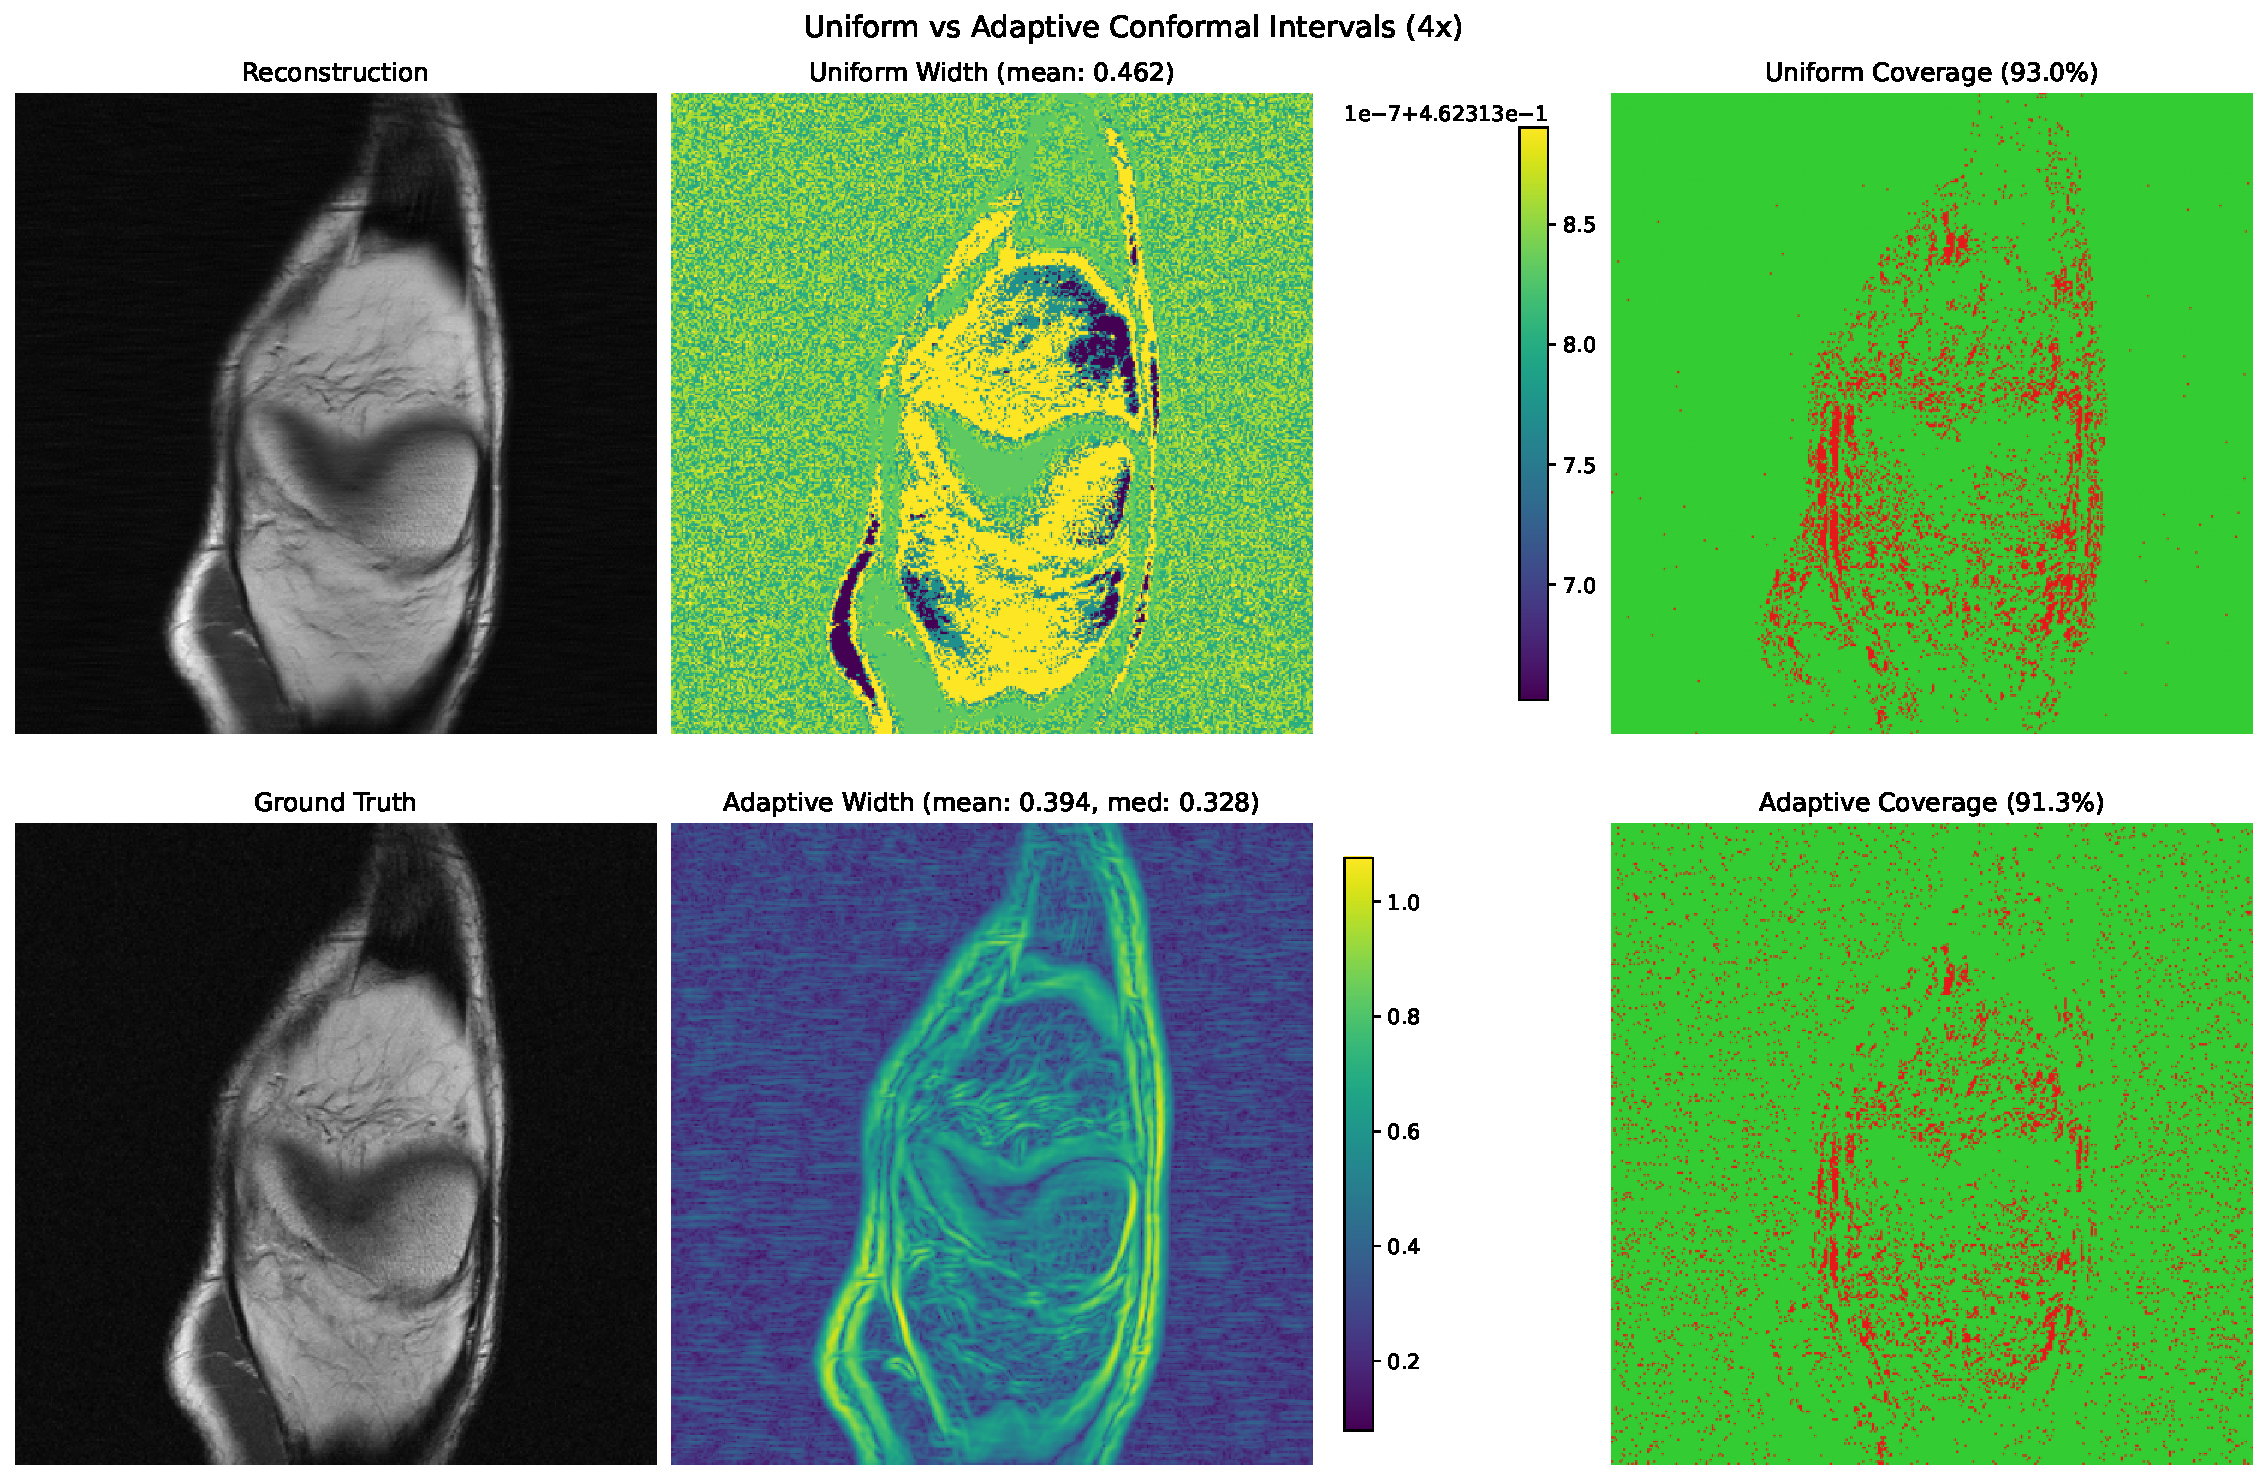
\includegraphics[width=0.95\textwidth]{figures/fig_adaptive_vs_uniform_4x.pdf}
    \caption{Uniform vs adaptive conformal intervals ($4{\times}$, 90\% nominal). Top: uniform, constant width across all pixels. Bottom: adaptive, tight in smooth regions, wide at anatomical boundaries. Both achieve ${\sim}90\%$ coverage.}
    \label{fig:adaptive}
\end{figure}

\subsection{K-Space Consistency Results}

Per-pixel k-space residuals show moderate spatial correlation with reconstruction errors ($r{=}0.39$ at $4{\times}$, $r{=}0.28$ at $8{\times}$). At the \emph{image level}, consistency scores correlate strongly with reconstruction error ($r{=}0.89$ at $4{\times}$, $r{=}0.80$ at $8{\times}$), reliably identifying poorly reconstructed images. Lower correlations at $8{\times}$ reflect fewer acquired k-space locations.

\paragraph{Relationship to conformal prediction.} Per-image CP coverage and k-space consistency score are moderately correlated ($r{=}{-}0.69$ at $4{\times}$, $r{=}{-}0.49$ at $8{\times}$), confirming partial overlap. However, they operate at different levels---CP provides \emph{pixel-wise statistical guarantees} while k-space consistency provides a \emph{physics-based spatial error map} and image-level flag---making them complementary in kind rather than redundant in information.

%----------------------------------------------------------------------
\section{Discussion}
\label{sec:discussion}
%----------------------------------------------------------------------

\paragraph{Interval width and coverage gap.} Our conformal guarantee is \emph{marginal}---it holds on average but can hide local miscoverage at edges. Adaptive intervals partially address this: the smooth--edge gap drops from 13.5\,pp to 0.2\,pp at $4{\times}$ (Table~\ref{tab:region_coverage}), though this does not achieve conditional coverage formally~\cite{angelopoulos2022image}. The absolute widths remain large (median 0.393 at $4{\times}$, ${\sim}40\%$ of dynamic range), reflecting the vanilla U-Net's reconstruction error; a stronger model~\cite{hammernik2018varnet,sriram2020e2evarnet} or learned nonconformity scores~\cite{angelopoulos2022image} would produce narrower intervals.

\paragraph{Difficulty modulator choice.} Gradient magnitude provides ${\sim}60{\times}$ spatial contrast (P90/P10), compared to MC Dropout's ${\sim}3.5{\times}$ at $p{=}0.05$. Even at $99\%$ nominal, MC Dropout achieves only $72\%$ empirical coverage (Figure~\ref{fig:calibration}a), so reaching $90\%$ would require intervals far exceeding CP's width---confirming that variance estimates at $p{=}0.05$ carry little spatial information~\cite{gal2016dropout,kuleshov2018calibration}.

\paragraph{The role of $\gamma$.} The ablation in Table~\ref{tab:gamma_ablation} reveals a clear transition: at $\gamma{<}0.3$, edges remain undercovered (positive gap); at $\gamma{>}0.3$, smooth regions become undercovered (negative gap) as raw gradient values create excessively wide intervals at boundaries. On this test split, the crossover near $\gamma{=}0.3$ gave the best observed trade-off. We note that $\gamma$ was selected on the test set---a proper protocol would use a separate validation split, and the crossover criterion (minimising $|\text{gap}|$) could automate this selection entirely.

\paragraph{Towards clinical use.} The proposed CP and k-space checks are post-hoc, requiring only a single deterministic forward pass plus lightweight residual computations, unlike MC Dropout which requires $T$ stochastic passes. In practice, the adaptive width map serves as an attention guide---highlighting unreliable regions for closer inspection. The k-space consistency score provides a complementary image-level flag for re-acquisition decisions. We evaluated on normal anatomy only; pathological cases (meniscal tears, tumours) warrant dedicated investigation, as these are precisely where clinical trust matters most.

\paragraph{Per-image coverage failures.} While marginal coverage holds on average, 3.8\% of test images at $4{\times}$ (2.3\% at $8{\times}$) fall below 80\% coverage. These cluster by MRI volume---the worst 10 images come from only 3--4 volumes---reflecting that slices from an anatomically atypical scan violate the exchangeability assumption together. Per-image coverage correlates with reconstruction quality ($r{=}0.68$): images that are hard to reconstruct (low PSNR) are also poorly covered, because the uniform conformal quantile $\hat{q}$ is set for the ``average'' image and is insufficient for outliers. Notably, adaptive CP does not rescue these cases (the worst image drops from 56.5\% to 51.1\% adaptive coverage), because it redistributes width spatially but does not increase the total budget. This motivates future work on image-conditional conformal prediction~\cite{angelopoulos2023gentle} or flagging low-coverage images via the k-space consistency score.

\paragraph{Limitations.} The k-space residual checks only \emph{acquired} locations ($25\%$ at $4{\times}$, $12.5\%$ at $8{\times}$), so null-space hallucinations~\cite{bhadra2021hallucinations} are undetectable. For models with built-in data consistency~\cite{hammernik2018varnet,schlemper2018cascade}, the residual would be near-zero by construction.

%----------------------------------------------------------------------
\section{Conclusion}
%----------------------------------------------------------------------

We presented two complementary mechanisms for trustworthy MRI reconstruction: split conformal prediction for pixel-wise intervals with marginal coverage guarantees (${\sim}90\%$ where MC Dropout, as an illustrative comparator at its reconstruction-optimal dropout rate, achieves only ${\sim}55\%$), and k-space residuals for range-space consistency checking. Using gradient magnitude as a spatial difficulty modulator, adaptive intervals reduce median width by ${\sim}15\%$ while maintaining marginal coverage. All methods are post-hoc and model-agnostic, requiring no retraining---a promising direction for clinical trust, though validation on pathological anatomy and stronger baselines remains necessary.

\bibliographystyle{splncs04}
\bibliography{references}

\end{document}
